\section{Third Exercise}
\subsection*{(a)}
\begin{figure}[h]
	\centering
	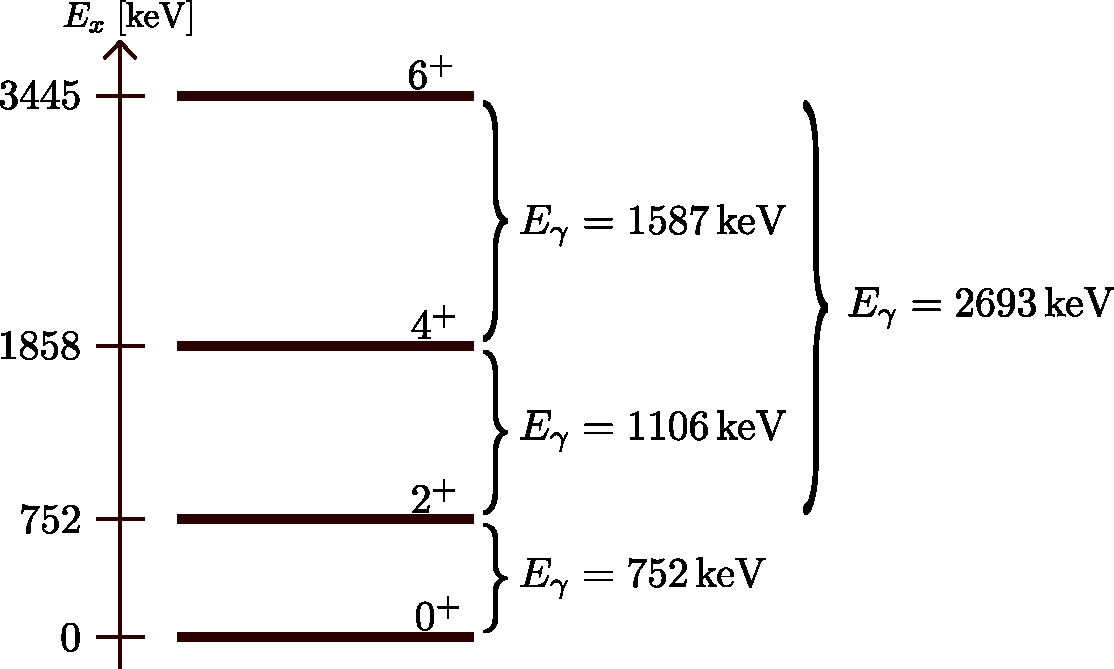
\includegraphics[width=0.8\textwidth]{./figures/level_sequence.pdf}
	\caption{The level sequence of $\nuc{Cr}{48}{24}$.}
	\label{fig:levels}
\end{figure}

\subsection*{(b)}
\paragraph{Solution:} The energy for a rotational state is given by
\begin{equation}
	E = \frac{\hbar^2 I (I+1)}{2 \mathcal{I}},
\end{equation}
then we get that
\begin{align}
	E_\gamma &= E(I+2) - E(I) = \frac{\hbar^2 (I + 2)(I+3)}{2 \mathcal{I}} - \frac{\hbar^2 I(I+1)}{2 \mathcal{I}}\\
	&= \frac{\hbar^2}{2 \mathcal{I}}[(I+2)(I+3) - I(I+1)] = \frac{\hbar^2}{2 \mathcal{I}} [(I^2 + 5I + 6)- (I^2 + I)]\\ 
	&= \frac{\hbar^2(4I + 6)}{2 \mathcal{I}} = \frac{\hbar^2(2I + 3)}{ \mathcal{I}}
\end{align}
Thus,
\begin{equation}
	E_\gamma = \frac{\hbar^2(2I + 3)}{ \mathcal{I}}. \label{eq:EI}
\end{equation}

\subsection*{(c)}
\paragraph{Solution:} Solving for $\mathcal{I}$ in Eq. \eqref{eq:EI} we obtain
\begin{equation}
	\mathcal{I} = \frac{\hbar^2(2I + 3)}{E_\gamma}.
\end{equation}
Using the values from Fig. \ref{fig:levels} we get for $I = 0, 2, 4$ the moment of inertias
\begin{align}
	\mathcal{I}_0 &= \SI{3.99}{\hhmev}\\
	\mathcal{I}_2 &= \SI{6.33}{\hhmev}\\
	\mathcal{I}_4 &= \SI{6.93}{\hhmev},
\end{align}
which gives an average moment of inertia $\langle \mathcal{I} \rangle = \SI{5.75}{\hhmev}$.

\paragraph{Answer:} The average moment of inertia for the rotational band of $\nuc{Cr}{48}{24}$ is $\langle \mathcal{I} \rangle = \SI{5.75}{\hhmev}$.

\subsection*{(d)}
\paragraph{Solution:} From the lectures we know that the theoretical moment of inertia for a rigid body nuclei is 
\begin{equation}
	\mathcal{I}_\mathrm{rigid} \approx \frac{2}{5} M r_0^2 A^{2/3} (1 + 0.31 \beta_2),
\end{equation}
where $M$ is the mass, $A$ is the atomic number, $r_0 \approx \SI{1.2}{\femto\meter}$ and $\beta_2 \approx 0.35$ is the quadrupole deformation parameter.
\begin{equation}
	\mathcal{I}_\mathrm{rigid} \approx \SI{128.80}{\hhmev}
\end{equation}

I think I do the conversion wrong to get the answer in the correct units. I don't have time to fix it :)